\subsection{States and Rules}
The agent operates within a predefined \textbf{6x6 grid-based maze} that consists of four distinct types of cells:

\begin{itemize}
    \item \textbf{Reward Cells (+1):} These cells provide a positive reward when the agent enters them.
    \item \textbf{Penalty Cells (-1):} These cells impose a negative reward on the agent.
    \item \textbf{Wall Cells (Impassable):} These act as obstacles; the agent cannot enter them.
    \item \textbf{Empty Cells (-0.05):} These cells apply a small penalty to encourage efficient navigation.
\end{itemize}

\vspace{5pt} % Add spacing before the next section

\noindent The environment follows these rules:

\begin{itemize}
    \item The agent cannot move into a wall or go out of bounds.
    \item There are no terminal states; the agent's state sequence continues indefinitely.
    \item At each step, the agent can perform one of four possible actions. 
\end{itemize}

\subsection{Possible Actions}
The agent can move in one of four cardinal directions (Up, Down, Left, Right).
However, due to \textbf{stochastic movement}, there is a chance that the agent does not move exactly as intended. Instead it may deviate in either direction perpendicular to the intended move.

\subsection{Transition Model}
The agent's movement follows a \textbf{probabilistic transition model}, introducing uncertainty into the decision-making:

\begin{itemize}
    \item \textbf{80\% probability} of moving in the intended direction.
    \item \textbf{10\% probability} of veering \textbf{right} (relative to the intended direction).
    \item \textbf{10\% probability} of veering \textbf{left} (relative to the intended direction).
    \item If the agent attempts to move into a wall or out of bounds, it remains in its current position.
\end{itemize}

\noindent This transition model simulates real-world uncertainties where actions may not always lead to expected outcomes, requiring the agent to adapt and plan accordingly.

\subsection{Discount Factor}
We are given the discount factor (gamma) of \textbf{0.99} for the scope of the assignment.

\subsection{Grid Implementation}
The Grid class creates an instance of the Grid environment. The Grid class accepts parameters as shown in Figure 1:

\begin{itemize}
    \item \textbf{tile\_reward}: a dictionary specifying the reward of each tile color.
    \item \textbf{map}: a 2-D array specifying the color of each tile.
    \item \textbf{values\_map}: a 2-D array of the initial values of each tile, with dimensions equal to that of \textbf{map}.
\end{itemize}

\vspace{10pt}  % Prevents formatting issues between list and figure

\begin{figure}[H]
    \centering
    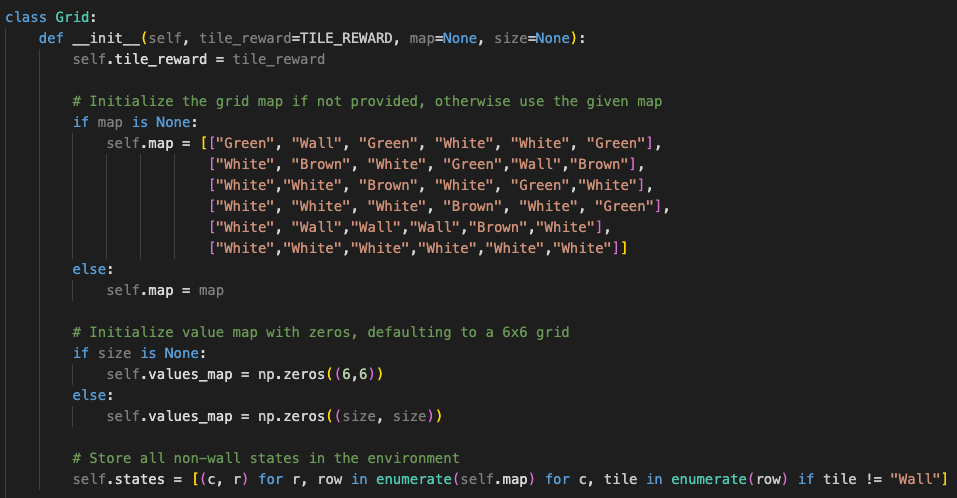
\includegraphics[width=0.8\textwidth]{images/grid_constructor.png}
    \caption{Grid Constructor Code Snippet}
    \label{fig:grid_environment}
\end{figure}

\noindent Due to how small the observation space was, we manually created a 2-D array for the 6x6 grid in Part 1. However, a function utilizing a nested-for loop was also implemented for custom grids.\vspace{10pt}

\noindent The \textit{step} method takes an action $a_t$ of the agent and updates the state from $s_t$ to $s_{t+1}$ and returns reward $r_t$. It provides a one-step lookahead for the utility values required in the Bellman update.

\begin{figure}[H]
    \centering
    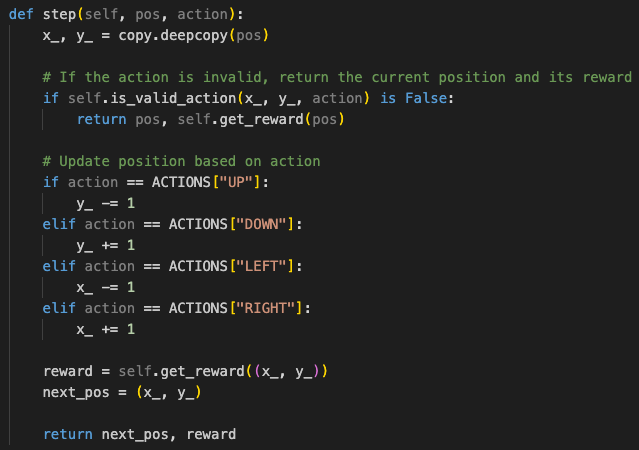
\includegraphics[width=0.8\textwidth]{images/step.png}
    \caption{\textit{step} method }
\end{figure}